\documentclass{beamer}
\usetheme{Berlin} % Bawcie się tym do woli
\usecolortheme{seahorse} % Bawcie się tym do woli
% Większość tych package'y to rzeczy które przeklejam z jakiejś starej templatki i pewnie nie wszystkie są potrzebne
\usepackage[polish]{babel}
\usepackage[utf8]{inputenc}
\usepackage[T1]{fontenc}
\usepackage{amsmath}
\usepackage{amssymb,amsfonts,amsthm}
\usepackage{multicol}
\usepackage{array}
\usepackage{geometry}
\usepackage{listings}
\usepackage{graphicx}
\usepackage{tabularx}
\usepackage{float}
\usepackage{hyperref}
\usepackage{mathspec} % wczytuje również fontspec
\setmainfont{Latin Modern Roman}
\setromanfont{Latin Modern Roman}
\setsansfont{Latin Modern Sans}
\setmonofont{Latin Modern Mono}
\setmathrm{Latin Modern Math}
\setmathfont(Digits,Latin)[Scale=MatchLowercase]{Latin Modern Math}
% \usepackage{minted} %To chyba package do wklejania kodu

\title{Porównanie algorytmów kryptograficznych RSA i Krzywej Eliptycznej}
\author{Autorzy:\\ Krzysztof Dąbrowski\\ Krzysztof Rudnik\\ Piotr Szczerba\\ Hussein Hazime\\ Jakub Więcław}
\date{2025-03-24}


\begin{document}

\begin{frame}
    \titlepage
\end{frame}

% Piotrek
\section{Wstęp}
\begin{frame}{Czym jest kryptografia asymetryczna}
    % Secure communications over insecure channels
\end{frame}

\begin{frame}{Jakie algortymy wybraliśmy}

\end{frame}
\begin{frame}{Pod jakimi kontami będziemy porównywać}

\end{frame}

\section{Sposoby działania wybranych algorytmów}
% Przedstawienie matematyki pod spodem i głównych idei wybranych algorytmów
\begin{frame}{Puzzle Merkle} % Krótka wspominka

\end{frame}
% ---------------------
% Hussein


\begin{frame}{RSA}

\end{frame}



\begin{frame}{ECC}

\end{frame}

% ---------------------
% KUBA

% Od tego momentu porównujemy algorytmy między sobą
\section{Zastosowania}

\subsection{Uwierzytelnianie}
\begin{frame}{Uwierzytelnianie}
    \begin{itemize}
        \pause
        \item Podpisy cyfrowe
        \pause
        \item Certifikaty
    \end{itemize}
\end{frame}

\begin{frame}{Podpisy cyfrowe - charakterystyka}
\pause
    \begin{itemize}
        \item Uwierzytelnianie nadawcy
        \pause
        \item Integralność danych
        \pause
        \item Niezaprzeczalność
    \end{itemize}
    
\end{frame}

\begin{frame}{Podpisy cyfrowe - metoda działania}
    \begin{columns}
        \column{0.5\textwidth}
        \textbf{RSA}
        \begin{itemize}
            \item Hashowanie wiadomości
            \item Szyfrowanie hashu kluczem prywatnym
            \item Odszyfrowanie hashu kluczem publicznym
            \item Porównanie hashy
        \end{itemize}

        \column{0.5\textwidth}
        \textbf{ECC (ECDSA)}
        \begin{itemize}
            \item Hashowanie wiadomości
            \item Generowanie losowej wartości $k$
            \item Obliczenie $(r, s)$
            \item Porównanie podpisu
        \end{itemize}
        \vspace{6pt}
    \end{columns}
\end{frame}

\begin{frame}{Certifikaty - budowa}
    \begin{itemize}
        \item Dane o właścicielu
        \item Klucz publiczny
        \item Podpis cyfrowy
        \item Okres ważności
        \item Algorytm podpisu
    \end{itemize}

\end{frame}

\begin{frame}{Certifikaty - działanie}
    \begin{itemize}
        \item Wysłanie certyfikatu do serwera
        \item Serwer sprawdza ważność i poprawność certyfikatu
        \item Po pozytywnej weryfikacji serwer szyfruje sesję i kontynuuje komunikację
    \end{itemize}
    
\end{frame}

\begin{frame}{Certyfikaty - algorytmy}

    \begin{columns}
        \column{0.5\textwidth}
        \centering
        
        \textbf{RSA}
        \begin{itemize}
            \item Powszechnie stosowany historycznie
            \item Większe klucze $\rightarrow$ większe wymagania sprzętowe
        \end{itemize}
        
        \column{0.5\textwidth}
        \centering

        \textbf{ECC}  
        \begin{itemize}
            \item Coraz popularniejszy
            \item Krótsze klucze $\rightarrow$ mniejsze wymagania sprzętowe
        \end{itemize}
        \vspace{7.5pt}

    \end{columns}

\end{frame}


\subsection{}
\begin{frame}{Kryptowaluty}
    \begin{center}
        \begin{minipage}{0.24\textwidth}
            \centering
            
\includegraphics[width=\linewidth]{applications/graphics/Bitcoin.png} \\
            \tiny{Źródło: \href{https://commons.wikimedia.org/wiki/File:Bitcoin_logo.svg}{commons.wikimedia.org}}
        \end{minipage}
        \hfill
        \begin{minipage}{0.24\textwidth}
            \centering
            
\includegraphics[width=\linewidth]{applications/graphics/Ethereum.png} \\
            \tiny{Źródło: \href{https://camo.githubusercontent.com/1b3d0063d6a8bcd56ca07b0ea2ef0f71b17a0fa8/687474703a2f2f737667706f726e2e636f6d2f6c6f676f732f657468657265756d2e737667}{camo.githubusercontent.com}}
        \end{minipage}
        \hfill
        \begin{minipage}{0.24\textwidth}
            \centering
            
\includegraphics[width=\linewidth]{applications/graphics/Dogecoin.png} \\
            \tiny{Źródło: \href{https://altcoinsbox.com/dogecoin-logo/}{altcoinsbox.com}}
        \end{minipage}
        \hfill
        \begin{minipage}{0.24\textwidth}
            \centering
            
\includegraphics[width=\linewidth]{applications/graphics/Litecoin.jpg} \\
            \tiny{Źródło: \href{https://cryptologos.cc/litecoin}{cryptologos.cc}}
        \end{minipage}
    \end{center}
\end{frame}



\begin{frame}{Komunikatory E2E - metoda działania}
    \begin{itemize}
        \item Wiadomości są widoczne tylko dla nadawcy i odbiorcy
        \item Klucz publiczny jest przesyłany do serwera
        \item Serwer przesyła klucz publiczny do odbiorcy
        \item Odbiorca odszyfrowuje wiadomość kluczem prywatnym
    \end{itemize}
\end{frame}
\begin{frame}{Komunikatory E2E - przykłady}
    \begin{center}
        \begin{minipage}{0.1\textwidth}
            
\includegraphics[width=\textwidth]{applications/graphics/Signal.png}
        \end{minipage}
        \begin{minipage}{0.6\textwidth}
            \textbf{X3DH oraz Curve25519}
        \end{minipage}

        \vspace{0.3cm}

        \begin{minipage}{0.1\textwidth}
            
\includegraphics[width=\textwidth]{applications/graphics/WhatsApp.png}
        \end{minipage}
        \begin{minipage}{0.6\textwidth}
            \textbf{Curve25519}
        \end{minipage}

        \vspace{0.3cm}

        \begin{minipage}{0.1\textwidth}
            
\includegraphics[width=\textwidth]{applications/graphics/Messenger.png}
        \end{minipage}
        \begin{minipage}{0.6\textwidth}
            \textbf{Signal Protocol}
        \end{minipage}

        \vspace{0.3cm}

        \begin{minipage}{0.1\textwidth}
            
\includegraphics[width=\textwidth]{applications/graphics/Imessage.png}
        \end{minipage}
        \begin{minipage}{0.6\textwidth}
            \textbf{RSA-2048 oraz ECDSA/ECDH}
        \end{minipage}
    \end{center}
\end{frame}

\begin{frame}{IoT}
    \begin{itemize}
        \item Uwierzytelnianie urządzeń (RSA/ECC)
        \item Szyfrowanie komunikacji (TLS, MQTT-TLS)
        \item Bezpieczne aktualizacje OTA
    \end{itemize}
\end{frame}

% ---------------------
% Krzysiek D
\section{Bezpieczeństwo}
% Porównanie bezpieczeństwa algorytmów RSA i ECC w zastosowaniu na aktualnymi technologiami

% Jak porównywać bezpieczeństwo algorytmów
\begin{frame}{Porównywanie bezpieczeństwa}
\textbf{Bity bezpieczeństwa \cite{BitSecurityOfCryptographicPrimitives}}
\pause
\begin{itemize}
    \pause
    \item Pojedyncza liczba
    \pause
    \item \( x = \log_2(N) \)
    \item \( x \) - liczba bitów bezpieczeństwa
    \item \( N \) - średnia ilość operacji wymaganych do złamania szyfru
\end{itemize}
\pause
\vspace{8mm}

\textit{Algorytm o sile 20 bitów bezpieczeństwa wymaga średnio $2^{20} = 1048576$ operacji do złamania.}

\end{frame}

\begin{frame}{Bezpieczeństwo RSA}
% Wielkość klucza to ilość bitów modułu n = p*q
Najszybszy klasyczny \footnote{tz. nie korzystający z matematyki kwantowej} algorytm refaktoryzacji liczb to Ogólne sito ciała liczbowego (GNFS) \footnote{ang. General Number Field Sieve}.
\pause
\begin{itemize}
    \item Złożoność \cite{GNFSImplementation} \begin{footnotesize}$$L(n) = \exp\left(\left(\frac{64}{9}\right)^{1/3} (\ln n)^{1/3} (\ln \ln n)^{2/3}\right)$$\end{footnotesize}
    \pause
    \item Liczba bitów bezpieczeństwa $= \log_2(L(n))$
\end{itemize}
\pause
$$
\begin{array}{|c|c|}
\hline
\textbf{Wielkość \, klucza \, RSA \, (bity)} & \textbf{Bity \, Bezpieczeństwa} \\
\hline
1024 & \sim 80 \\
2048 & \sim 112 \\
3072 & \sim 128 \\
\hline
\end{array}
$$
\end{frame}

\begin{frame}{Bezpieczeństwo ECC}
% Wielkość klucza to rozmiar jednego wymiaru dyskretnej przestrzeni
Najszybszy klasyczny \footnote{tz. nie korzystający z matematyki kwantowej} algorytm do rozwiązania ECDLP to algorytm faktoryzacji rho Pollarda \cite{SolvingECDLP}.
\pause
\begin{itemize}
    \item Dla przestrzeni wielkości k wymaga $\sqrt{k}$ kroków
    \item Do x bitów bezpieczeństwa potrzebny jest klucz wielkości 2x
    \pause
    \item Przykładowo 256-bitowa krzywa teoretycznie daje 128-bitów bezpieczeństwa
\end{itemize}
\pause
Rzeczywiste bezpieczeństwo $\approx 0.886*\sqrt{k}$
\pause
\begin{itemize}
    \item \textit{secp256k1} klucz 256 bit $\Rightarrow$ 127.8 bitów bezpieczeństwa \cite{Secp256k1Security}
    \item \textit{Curve448} klucz 448 bit $\Rightarrow$ 222.8 bitów bezpieczeństwa \cite{Secp256k1Security}
\end{itemize}
% Rzeczywiste bezpieczeństwo jest mniejsze, ponieważ ranga krzywej w dyskretnej przestrzeni jest zazwyczaj mniejsza niż wielkość pojedynczego wymiaru przestrzeni

\end{frame}

\begin{frame}{Porówanie długości klucza}
    \begin{figure}
        \centering
            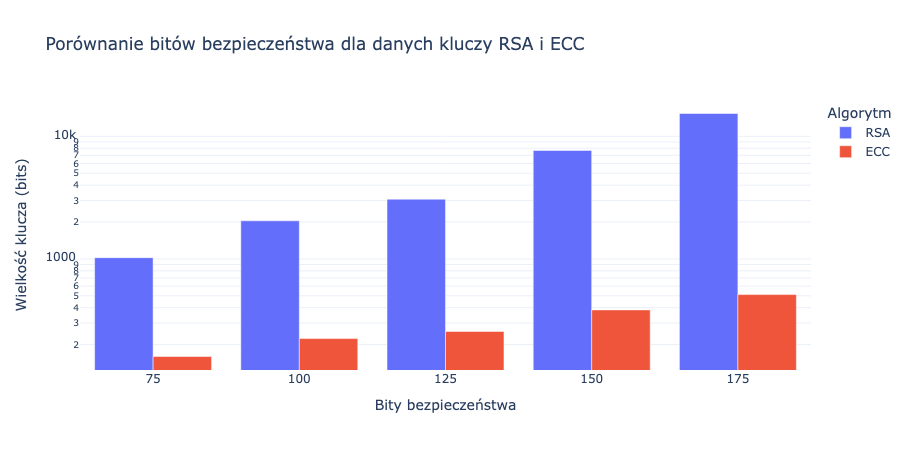
\includegraphics[width=\textwidth]{security/graphics/Porównanie bitów bezpieczeństwa dla danych kluczy RSA i ECC}
            \caption{Porównanie bitów bezpieczeństwa dla danych kluczy RSA i ECC}
    \end{figure}
\end{frame}

\begin{frame}{Podatności ECC}
\framesubtitle{Podatne implementacje}
\textbf{$ECDLP \neq ECC$} \\
\pause
Bezpieczne implementacje są teoretycznie możliwe. \\
\pause
Implementacja może być podatna na \cite{SafeCurves}
\begin{itemize}
    \item Ataki na generator liczb losowych
    \item Błędne wyniki dla specyficznych punktów
    \item Wyciek informacji, gdy podany punkt nie należy do krzywej
    \item Ataki poprzez pomiar czasu wykonania
\end{itemize}
\pause
\vspace{3mm}
Przykład: Wyciek kluczy prywatnych Sony PlayStation 3 w 2010 \cite{ConsoleHacking2010}
% W 2010 roku odkryto, że implementacja ECDSA w PlayStation 3 miała poważny błąd.
% Błąd polegał na używaniu tej samej wartości nonce dla różnych podpisów.
% Pozwoliło to na odzyskanie klucza prywatnego z dwóch podpisów cyfrowych.
% W wyniku tego ataku możliwe było uruchamianie nieautoryzowanego oprogramowania na konsoli.
\end{frame}

\begin{frame}{Podatności ECC}
\framesubtitle{Podatne krzywe}
Nie wszystkie krzywe gwarantują, że ECDLP jest trudny.
Ataki na podatne krzywe \cite{WeakCurvesInEllipticCurveCryptography}
\begin{itemize}
    \item Algorytm Pohinga-Hellmana
    \item Algorytm Smarta
\end{itemize}
\pause
\vspace{3mm}
Możliwe jest \textbf{celowe wybranie słabej krzywej} jako backdoor.
\end{frame}

\begin{frame}{Podatności ECC}
    \framesubtitle{Bezpieczny system}
    Standardy wyboru krzywych \cite{SafeCurves}
    \begin{scriptsize}
        \begin{itemize}
            \item ANSI X9.62 (1999)
            \item IEEE P1363 (2000)
            \item SEC 2 (2000)
            \item NIST FIPS 186-2 (2000)
            \item ANSI X9.63 (2001)
            \item Brainpool (2005)
            \item NSA Suite B (2005)
            \item ANSSI FRP256V1 (2011)
        \end{itemize}
    \end{scriptsize}
    \pause
    \vspace{3mm}
    Wśród przebadanych krzywych są też bardziej wydajne krzywej z mniejszym bezpieczeństwem dla tej samej długości klucza. \cite{PracticalCryptographyForDevelopers}
\end{frame}

\begin{frame}{Ataki na RSA}
\begin{itemize}
    \item Ataki kanału bocznego
    \item Ataki na generator liczb losowych
    \pause
    \item \textbf{Podatne liczby pierwsze}
    \pause
    \item \textbf{Długość klucza}
\end{itemize}
Klucze długości 1024 bit są dziś niewystarczająco bezpieczne.
\end{frame}

\begin{frame}{Użycie bibliotek}
\pause
\begin{figure}
    \centering
        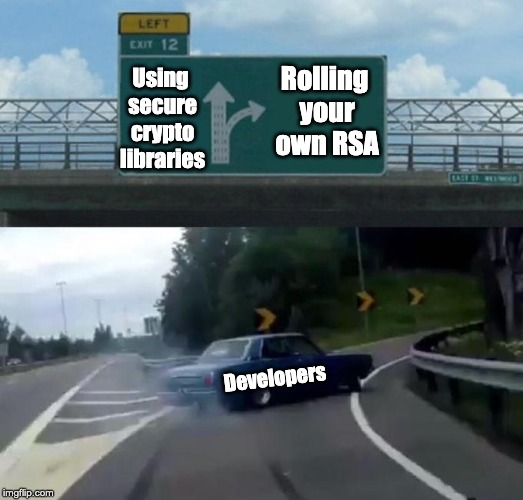
\includegraphics[height=0.55\textwidth]{security/graphics/developer-implements-rsa-car-meme}
        \caption{Źródło: \cite{SeriouslyStopUsingRsa}}
\end{figure}
\end{frame}

% ---------------------
% Krzysiek R
\section{Przyszłość}
\begin{frame}{ECC jest łatwiejsze do złamania przez algorytm Shore'a niż RSA}

\end{frame}
\begin{frame}{Bell's Theorem} % Opcjolanlne

\end{frame}

\begin{frame}{Regulacje prawne}

\end{frame}

\end{document}
